\section{Ape 1}

\subsection{Vrai ou Faux}
\begin{enumerate}
	\item{L'élimination d'un sommet de degré maximum peut augmenter le degré moyen d'un graph.}
	\item{Un graph qui ne contient pas de triangle est pibarti}
	\item{Deux graphes qui possèdent un même nombre de sommets et dont les listes de degrés sont identiques sont isomorphes. Même question, si, en plus, les graphes sont connexes.}
	\item{Un graphe simple de 2 sommets au moins possède toujours 2 sommets de degré identiques}
	\item{$\exists$ un graph simple dont les degrés des sommets sont $\{1,2,2,3,3,4\}$}
	\item{$\exists$ un graph simple dont les degrés des sommets sont $\{1,1,1,2,3,4,6\}$}	
\end{enumerate}

\subsection{Démontrez}
\begin{enumerate}
\item{D'un sommet de degré impair, $\exists$ toujours un chemin jusqu'à un autre sommet de degré impair.}
\item{Pour un graph simple et connexe de n sommets, on a $(n-1) \leq |E| \leq \frac{n \times (n-1)}{2}$}
\item{Un graphe simple qui possède plus de $\frac{(n-1) \times (n-2)}{2}$ arêtes est connexe.}
\item{Tout graphe qui possède n sommets et h arêtes possède au moins $n-k$ composantes connexes}
\end{enumerate}

\subsection{Graphe de l'hypercube}
Soit $G_{i}$ le graphe dont les sommets sont des k-tuples de 0 et 1. Deux sommets de G sont adjacents si leurs k-tuples ne diffèrent qu'en une seule position. Montrez que le graphe est biparti, k-régulier et donnez son nombre arrêtes.

\subsection{Parcours fermés}
\begin{enumerate}
\item{Comptez le nombre de parcours fermés de longueur k dans $K_{n}$}
\item{Comptez le nombre de parcours fermés de longueur k dans $K_{k,n}$}
\end{enumerate}

\subsection{Trouvez le nombre de parcours de longueur k du sommet A à lui-même.}
\begin{figure}
\center
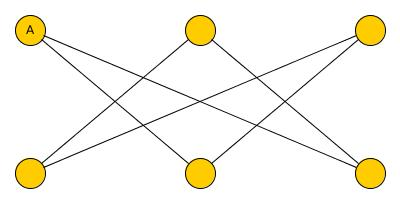
\includegraphics[scale=0.5]{graph_ape1_ex5}
\end{figure}

\subsection{Démonstration - Les rois du graphe}
Un tournoi de n joueurs est un graphe complet $K_{n}$ dans lequel on a choisi une direction pour chaque arête. $\exists$ une arête $(u,v)$ lorsque u a remporté sa partie contre v. Un sommet u d'un tournoi est un roi si quel que soit le sommet v du graphe, il y a une arête $(u,v)$ où il a une arête intermédiaire w et des arêtes $(u,w)$ et $(w,v)$.

Prouvez qu'il existe toujours au moins un roi.
Utiliser ce résultat pour montrer que dans le cas où aucun sommet n'a un degré entrant nul, il y a toujours au moins 2 rois.


